\documentclass[tikz,border=10pt]{standalone}
% Shared look for every TikZ diagram. Load with % Shared look for every TikZ diagram. Load with % Shared look for every TikZ diagram. Load with \input{../../tools/tikz-style.tex}
\usepackage[T1]{fontenc}
\usepackage{lmodern}
\renewcommand{\sfdefault}{lmr}  % diagrams use the same serif as the text
\usetikzlibrary{arrows.meta, positioning, shapes.geometric, calc, fit, backgrounds}
\definecolor{cblue}{HTML}{4C78A8}
\definecolor{corange}{HTML}{F58518}
\definecolor{cgreen}{HTML}{54A24B}
\definecolor{cred}{HTML}{E45756}
\definecolor{cpurple}{HTML}{B279A2}
\definecolor{cgrey}{HTML}{6B6B6B}
\tikzset{
  every picture/.style={font=\sffamily, line width=1.2pt},
  box/.style={draw=#1, fill=#1!12, rounded corners=4pt, align=center, inner sep=7pt, minimum height=1.1cm},
  box/.default=cgrey,
  arrow/.style={-{Stealth[length=3mm]}, draw=cgrey, line width=1.4pt},
  title/.style={font=\sffamily\bfseries\Large},
  note/.style={font=\sffamily\small, text=cgrey, align=center},
}
\AtBeginDocument{\hyphenpenalty=10000 \exhyphenpenalty=10000}

\usepackage[T1]{fontenc}
\usepackage{lmodern}
\renewcommand{\sfdefault}{lmr}  % diagrams use the same serif as the text
\usetikzlibrary{arrows.meta, positioning, shapes.geometric, calc, fit, backgrounds}
\definecolor{cblue}{HTML}{4C78A8}
\definecolor{corange}{HTML}{F58518}
\definecolor{cgreen}{HTML}{54A24B}
\definecolor{cred}{HTML}{E45756}
\definecolor{cpurple}{HTML}{B279A2}
\definecolor{cgrey}{HTML}{6B6B6B}
\tikzset{
  every picture/.style={font=\sffamily, line width=1.2pt},
  box/.style={draw=#1, fill=#1!12, rounded corners=4pt, align=center, inner sep=7pt, minimum height=1.1cm},
  box/.default=cgrey,
  arrow/.style={-{Stealth[length=3mm]}, draw=cgrey, line width=1.4pt},
  title/.style={font=\sffamily\bfseries\Large},
  note/.style={font=\sffamily\small, text=cgrey, align=center},
}
\AtBeginDocument{\hyphenpenalty=10000 \exhyphenpenalty=10000}

\usepackage[T1]{fontenc}
\usepackage{lmodern}
\renewcommand{\sfdefault}{lmr}  % diagrams use the same serif as the text
\usetikzlibrary{arrows.meta, positioning, shapes.geometric, calc, fit, backgrounds}
\definecolor{cblue}{HTML}{4C78A8}
\definecolor{corange}{HTML}{F58518}
\definecolor{cgreen}{HTML}{54A24B}
\definecolor{cred}{HTML}{E45756}
\definecolor{cpurple}{HTML}{B279A2}
\definecolor{cgrey}{HTML}{6B6B6B}
\tikzset{
  every picture/.style={font=\sffamily, line width=1.2pt},
  box/.style={draw=#1, fill=#1!12, rounded corners=4pt, align=center, inner sep=7pt, minimum height=1.1cm},
  box/.default=cgrey,
  arrow/.style={-{Stealth[length=3mm]}, draw=cgrey, line width=1.4pt},
  title/.style={font=\sffamily\bfseries\Large},
  note/.style={font=\sffamily\small, text=cgrey, align=center},
}
\AtBeginDocument{\hyphenpenalty=10000 \exhyphenpenalty=10000}

\begin{document}
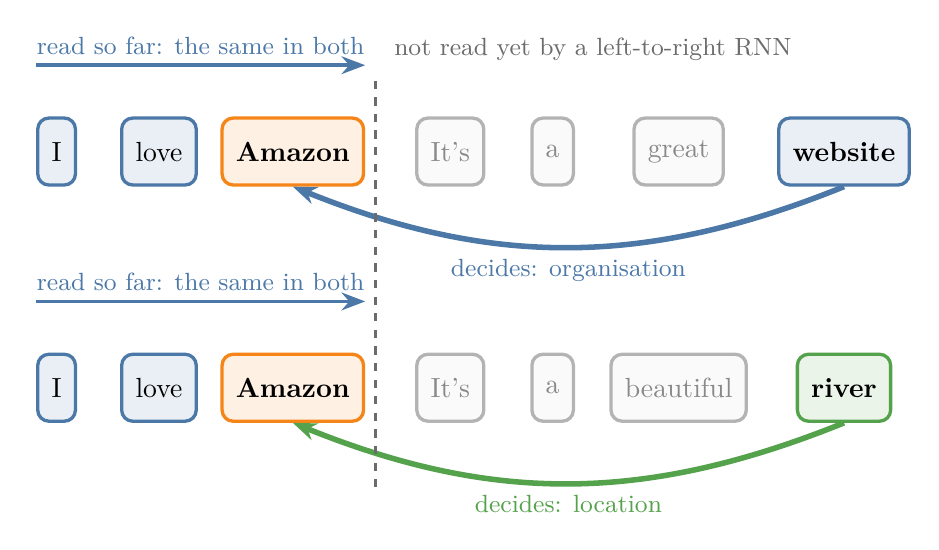
\begin{tikzpicture}[w/.style={box=cblue, inner sep=5pt, minimum height=0.85cm, font=\sffamily},
  fut/.style={box=cgrey, inner sep=5pt, minimum height=0.85cm, font=\sffamily, draw opacity=0.5, fill opacity=0.3, text opacity=0.45},
  am/.style={box=corange, inner sep=5pt, minimum height=0.85cm, font=\sffamily\bfseries}]
  \foreach \y/\last/\lab/\col/\adj in {0/website/organisation/cblue/great, -3.0/river/location/cgreen/beautiful} {
    \pgfmathtruncatemacro\k{\y<0}
    \node[w] (a\k) at (0,\y) {I};
    \node[w] (b\k) at (1.3,\y) {love};
    \node[am] (c\k) at (3.0,\y) {Amazon};
    \node[fut] (d\k) at (5.0,\y) {It's};
    \node[fut] (e\k) at (6.3,\y) {a};
    \node[fut] (f\k) at (7.9,\y) {\adj};
    \node[box=\col, inner sep=5pt, minimum height=0.85cm, font=\sffamily\bfseries] (g\k) at (10.0,\y) {\last};
    \draw[arrow, draw=cblue] ([yshift=0.65cm]a\k.north west) -- node[above, note, text=cblue] {read so far: the same in both} ([yshift=0.65cm]c\k.north east);
    \draw[arrow, draw=\col, line width=2pt] (g\k.south) to[bend left=22] node[below, note, text=\col] {decides: \lab} (c\k.south);
  }
  \draw[cgrey, dashed] (4.05,0.9) -- (4.05,-4.3);
  \node[note, anchor=west] at (4.15,1.3) {not read yet by a left-to-right RNN};
\end{tikzpicture}
\end{document}
